\begin{fullwidth}
\section{Red Flags} % Top level section
\begin{enumerate}
    \item \textbf{Potential AI Chat-bot}
            \\\medskip
                \item[--] The interviewer, who is claiming to be human, is responding in a time frame that is unrealistic to expect from a real person.
            \\\medskip
                \item[--] When texting Sam was asked for certain keywords which would serve as a prompt for the chat-bot to generate text tailored to their current conversation \hyperref[sec:Fig7]{(See Figure 7)}.
            \\\medskip
    \item \textbf{Inconsistent Information}
            \\\medskip
                \item[--] Neither Mr. Bondeson, Mr. Manly, or Ms. McDaniel ever refer to HealthComp by it's new name, Personify Health.
            \\\medskip
                \item[--] The original interview offer Sam received was from HealthComp, LLC. Upon entering the interview, it was revealed that she was actually interviewing for a company called Omnicell \hyperref[sec:Fig8]{(See Figure 8)}. After reviewing public records, the team concluded that Omnicell is not affiliated with HealthComp or Personify Health whatsoever.
            \\\medskip
                \item[--] In the beginning of the interview, Mr. Manley introduces himself to be from Omincell, Inc., but  later switches to HealthComp, LLC. \hyperref[sec:Fig9]{(See Figure 9)}.
            \\\medskip
                \item[--] The job offer letter Sam received was for HealthComp, which was consistent with the initial email, but not with the text based interview.
    \item \textbf{Point of Contact Discrepancies}
            \\\medskip
                \item[--] As stated in the email sent from HealthComp, LLC, the point of contact for this interview was supposed to be Mr. David W. Bondeson; however, the interviewer introduces himself as Mr. Gavin Manley from Omnicell, Inc. despite having the contact name "david donbenson" in Teams \hyperref[sec:Fig10]{(See Figure 10)}.
            \\\medskip
                \item[--] In the interview, Mr. Manley Introduces himself to be from Omnicell, Inc., but according to his Linkedin profile, he's currently employed at Docusign as a Senior Enterpise Account Executive \hyperref[sec:Fig2]{(See Figure 2)}.
            \\\medskip
                \item[--] When introducing himself, Mr. Manley states that he received his Bachelor of Science in Electrical Engineering from the Swiss University of Applied Science, Winterthur \hyperref[sec:Fig11]{(See Figure 11)}. This information is inconsistent with Mr. Manley’s LinkedIn profile indicates that he received a Bachelor of Science in Business Administration from the University of Central Florida \hyperref[sec:Fig3]{(See Figure 3)}.
            \\\medskip 
                \item[--] During his time at Omnicell, Mr. Manley was a Medical Account Executive and not on the board of directors as he claims in the interview \hyperref[sec:Fig2]{(See Figure 2)}. 
            \\\medskip
                \item[--] Mr. Bondeson's title at HealthComp, LLC. is Director of Stop Loss sales and not Interview Manager \hyperref[sec:Fig4]{(See Figure 4)}.
            \\\medskip
                \item[--] Kellie McDaniel is not listed as a HealthComp employee
            \\\medskip
                \item[--] Email requests all communication be sent through a @healthcomp.live domain instead of the official @healthcomp.com domain listed on their Linkedin and website \hyperref[sec:Fig5]{(See Figure 5)}.
    \item  \textbf{Professionalism}
            \\\medskip
                \item[--] Numerous grammar \hyperref[sec:Fig12]{(See Figures 12-13)}, spelling \hyperref[sec:Fig14]{(See Figure 14)}, and convention errors \hyperref[sec:Fig15]{(See Figure 15)}.
            \\\medskip
                \item[--] Does not address recipient of email in interview offer letter and instead refers to Sam as Candidate and uses a verification code to track her application \hyperref[sec:Fig14]{(See Figure 16)}.
            \\\medskip
                \item[--] Email signed by HealthComp instead of the sender or an HR Representative \hyperref[sec:Fig16]{(See Figure 16)}.
                \item[--] Lack of branding on throughout all contact, most companies will usually include a header, footer, and logo in their emails. 
            \\\medskip            
                \item[--] The contact name on the Microsoft Teams chat reads, "david donbenson" and not "David Bondeson," lacking proper capitalization and spelling of the last name provided in the original email \hyperref[sec:Fig17]{(See Figure 17}). 
    \item   \textbf{Lure}
            \\\medskip
                \item[--] Offer letter states Sam will have to purchase her own office equipment from a supplied vendor and will be reimbursed, which is a common scam acknowledged by the Federal Trade Commission. The vendor could be one the scammers created themselves to have payment redirected towards them, and you wont receive the products ordered 
                \item[--] Employer requests a photo of Sam, which could be used for identity theft 
\end{enumerate}

\subsubsection{Red Flag Evidence}
    \begin{figure*}[H] % Use the figure* environment for full width figures
        \label{sec:Fig7}
        \centering
        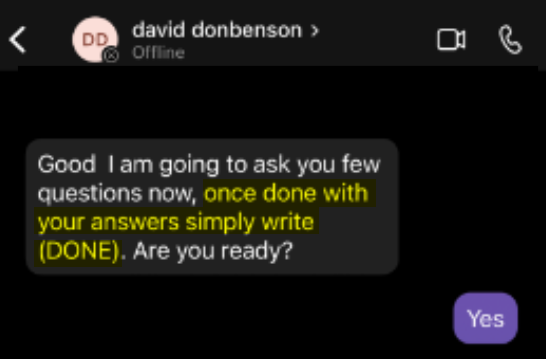
\includegraphics[width=.75\linewidth]{assets/chatbot.png}
        \captionsetup{justification=centering}
        \caption{The interviewer asked Sam to reply with "DONE" or other cue words at several points.}
    \end{figure*}

    \begin{figure*}[H] % Use the figure* environment for full width figures
        \label{sec:Fig8}
        \centering
        \begin{subfigure}{0.5\textwidth}
            \centering
            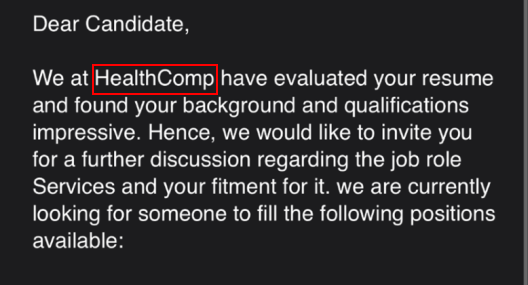
\includegraphics[width=1.37\linewidth]{assets/Healthcomp.png}
            \captionsetup{justification=centering}
            \caption{Initial Email from HealthComp, LLC.}
        \end{subfigure}
        \hfill
        \begin{subfigure}{0.5\textwidth}
            \centering
            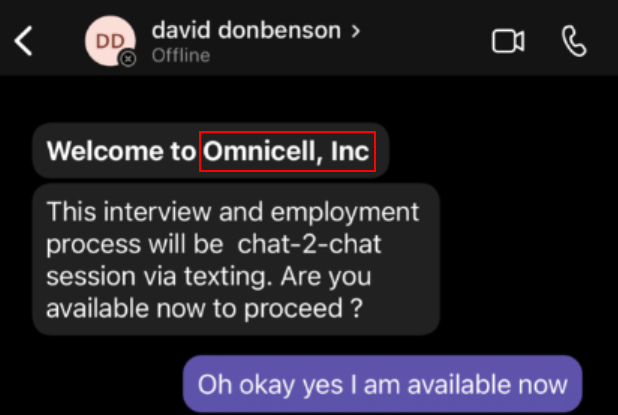
\includegraphics[width=1.37\linewidth]{assets/Omnicell.png}
            \captionsetup{justification=centering}
            \caption{Interview introduction as Omnicell, Inc.}
        \end{subfigure}
        \hfill
        \captionsetup{justification=centering}
        \caption{Discrepancy in the company offering the job.}
    \end{figure*}

    \begin{figure*}[H] % Use the figure* environment for full width figures
        \label{sec:Fig9}
        \centering
        \begin{subfigure}{0.5\textwidth}
            \centering
            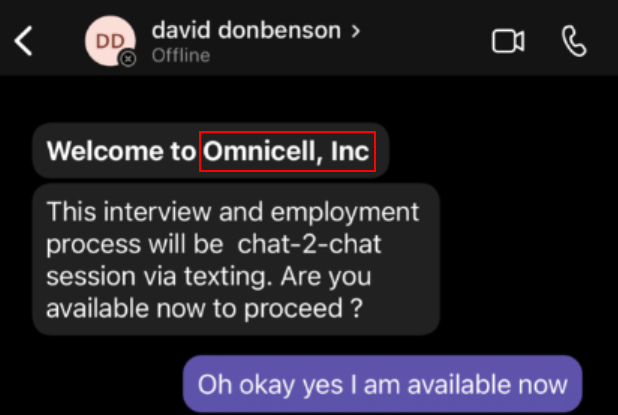
\includegraphics[width=1.37\linewidth]{assets/Omnicell.png}
            \captionsetup{justification=centering}
            \caption{Interview introduction as Omnicell, Inc.}
        \end{subfigure}
        \hfill
        \begin{subfigure}{0.5\textwidth}
            \centering
            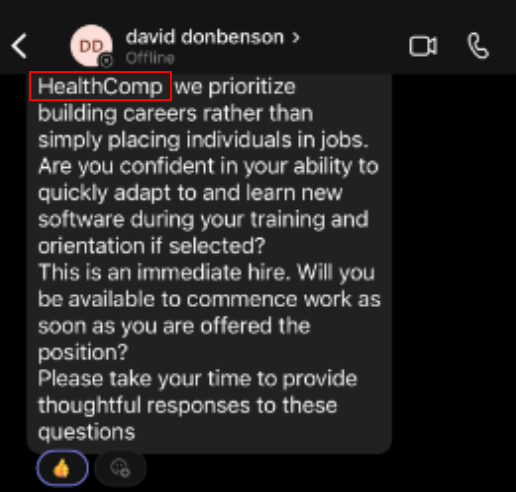
\includegraphics[width=1.37\linewidth]{assets/switchToHealthcomp.png}
            \captionsetup{justification=centering}
            \caption{HealthComp used later in the interview.}
        \end{subfigure}
        \hfill
        \captionsetup{justification=centering}
        \caption{The interviewer switches between HealthComp and Omnicell.}
    \end{figure*}


    \begin{figure*}[H] % Use the figure* environment for full width figures
        \label{sec:Fig10}
        \centering
        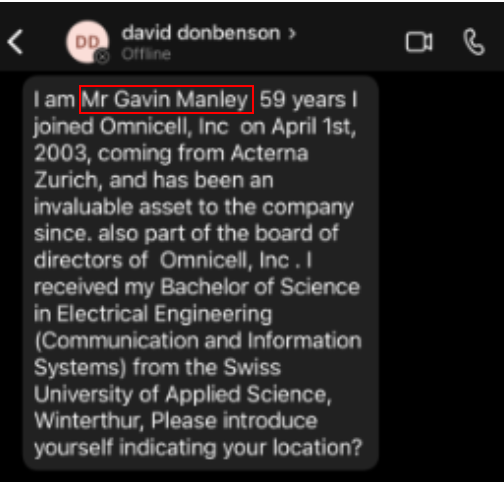
\includegraphics[width=.75\linewidth]{assets/ManelyIntroduction.png}
        \captionsetup{justification=centering}
        \caption{The interviewer introduces himself as Mr. Gavin Manley.}
    \end{figure*}

    \begin{figure*}[H] % Use the figure* environment for full width figures
        \label{sec:Fig11}
        \centering
        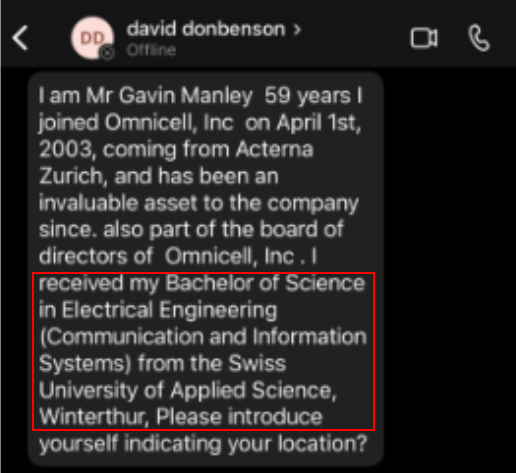
\includegraphics[width=.9\linewidth]{assets/ManleyInterviewCollege.png}
        \captionsetup{justification=centering}
        \caption{Mr. Manley claimed to have graduated from the Swiss University of Applied Science.}
    \end{figure*}

    \begin{figure*}[H] % Use the figure* environment for full width figures
        \label{sec:Fig12}
        \centering
        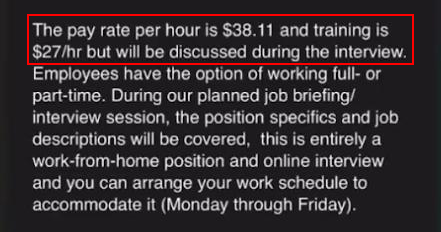
\includegraphics[width=.9\linewidth]{assets/missedCommas.png}
        \captionsetup{justification=centering}
        \caption{There should be a comma following "\$27/hr" and before "but"}
    \end{figure*}

    \begin{figure*}[H] % Use the figure* environment for full width figures
        \label{sec:Fig13}
        \centering
        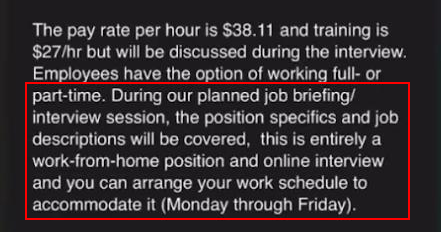
\includegraphics[width=.9\linewidth]{assets/runon.png}
        \captionsetup{justification=centering}
        \caption{This is a run-on sentence that should be broken up into two or three separate sentences.}
    \end{figure*}

    \begin{figure*}[H] % Use the figure* environment for full width figures
        \label{sec:Fig13}
        \centering
        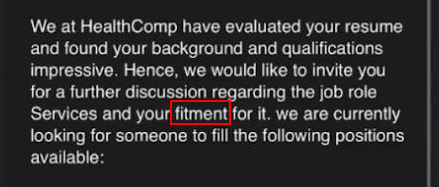
\includegraphics[width=.9\linewidth]{assets/misspelling.png}
        \captionsetup{justification=centering}
        \caption{Misspelling of "fitment". It should just say "fit".}
    \end{figure*}

    \begin{figure*}[H] % Use the figure* environment for full width figures
        \label{sec:Fig14}
        \centering
        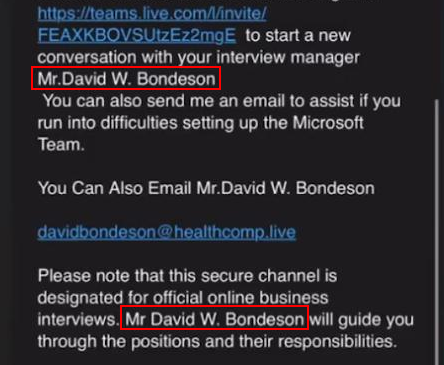
\includegraphics[width=.9\linewidth]{assets/titleerror.png}
        \captionsetup{justification=centering}
        \caption{Discrepancy between "Mr.David W. Bondeson" compared to "Mr David W. Bondeson".}
    \end{figure*}

    \begin{figure*}[H] % Use the figure* environment for full width figures
        \label{sec:Fig15}
        \centering
        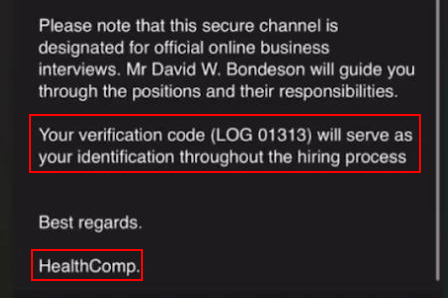
\includegraphics[width=.9\linewidth]{assets/VerificationCode.png}
        \captionsetup{justification=centering}
        \caption{Verification code to be used as identification and email signature from HealthComp}
    \end{figure*}

    \begin{figure*}[H] % Use the figure* environment for full width figures
        \label{sec:Fig16}
        \centering
        \begin{subfigure}{0.5\textwidth}
            \centering
            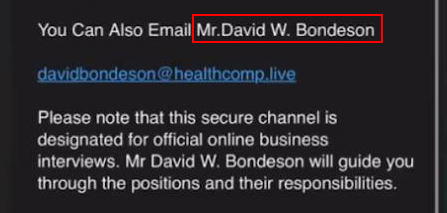
\includegraphics[width=1.37\linewidth]{assets/BondesonEmail.png}
            \captionsetup{justification=centering}
            \caption{Original email with correct spelling.}
        \end{subfigure}
        \hfill
        \begin{subfigure}{0.5\textwidth}
            \centering
            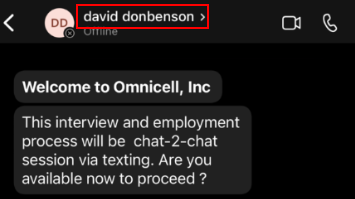
\includegraphics[width=1.37\linewidth]{assets/TeamsNamepng.png}
            \captionsetup{justification=centering}
            \caption{Misspelled name in Microsoft Teams interview.}
        \end{subfigure}
        \hfill
        \captionsetup{justification=centering}
        \caption{There is a clear misspelling between the point of contact and the Teams account hosting the interview.}
    \end{figure*}

\end{fullwidth}